%%%%%%%%%%%%%%%%%%%%%%%%%%%%%%%%%%%%%%%%%
% Short Sectioned Assignment
% LaTeX Template
% Version 1.0 (5/5/12)
%
% This template has been downloaded from:
% http://www.LaTeXTemplates.com
%
% Original author:
% Frits Wenneker (http://www.howtotex.com)
%
% License:
% CC BY-NC-SA 3.0 (http://creativecommons.org/licenses/by-nc-sa/3.0/)
%
%%%%%%%%%%%%%%%%%%%%%%%%%%%%%%%%%%%%%%%%%

%----------------------------------------------------------------------------------------
%	PACKAGES AND OTHER DOCUMENT CONFIGURATIONS
%----------------------------------------------------------------------------------------

\documentclass[titlepage, paper=a4, fontsize=11pt]{scrartcl} % A4 paper and 11pt font size

\usepackage[T1]{fontenc} % Use 8-bit encoding that has 256 glyphs
\usepackage{fourier} % Use the Adobe Utopia font for the document - comment this line to return to the LaTeX default
\usepackage[english]{babel} % English language/hyphenation
\usepackage{amsmath,amsfonts,amsthm} % Math packages
\usepackage{listings}

\usepackage{lipsum} % Used for inserting dummy 'Lorem ipsum' text into the template
\usepackage{graphicx}


\usepackage{sectsty} % Allows customizing section commands
\allsectionsfont{\centering \normalfont\scshape} % Make all sections centered, the default font and small caps

\usepackage{fancyhdr} % Custom headers and footers
\pagestyle{fancyplain} % Makes all pages in the document conform to the custom headers and footers
\fancyhead{} % No page header - if you want one, create it in the same way as the footers below
\fancyfoot[L]{} % Empty left footer
\fancyfoot[C]{} % Empty center footer
\fancyfoot[R]{\thepage} % Page numbering for right footer
\renewcommand{\headrulewidth}{0pt} % Remove header underlines
\renewcommand{\footrulewidth}{0pt} % Remove footer underlines
\setlength{\headheight}{13.6pt} % Customize the height of the header

\numberwithin{equation}{section} % Number equations within sections (i.e. 1.1, 1.2, 2.1, 2.2 instead of 1, 2, 3, 4)
\numberwithin{table}{section} % Number tables within sections (i.e. 1.1, 1.2, 2.1, 2.2 instead of 1, 2, 3, 4)

\setlength\parindent{0pt} % Removes all indentation from paragraphs - comment this line for an assignment with lots of text

%----------------------------------------------------------------------------------------
%	TITLE SECTION
%----------------------------------------------------------------------------------------

\newcommand{\horrule}[1]{\rule{\linewidth}{#1}} % Create horizontal rule command with 1 argument of height

\title{	
\normalfont \normalsize 
\textsc{University of Virginia} \\ [25pt] % Your university, school and/or department name(s)
\horrule{0.5pt} \\[0.4cm] % Thin top horizontal rule
\huge ECE/CS 5565 Midterm Exam \\ % The assignment title
\horrule{2pt} \\[0.5cm] % Thick bottom horizontal rule
}

\author{Shawn (Shuoshuo) Chen\\sc7cq@virginia.edu} % Your name

\date{\normalsize\today} % Today's date or a custom date

\begin{document}

\maketitle % Print the title

%----------------------------------------------------------------------------------------
%	PROBLEM 1
%----------------------------------------------------------------------------------------

\section*{Problem 1}
(a).
For one bit, there is almost no transmission delay, the only time it takes is to pass across two links.
So the propagation delay to send across the end-to-end path is $d_{prop}=2*0.5=1\ ms$. \\

(b).
Since the router is operating in store-and-forward mode, the delay adds up for two links. Consider the packet-level pipelining, the first packet needs $d_1$ time to travel across the path, where
\begin{align*} 
\begin{split}
d_1 &= 2*(d_{prop} + d_{trans}) \\
&= 2*(0.5 + 0.012) \\
&= 1.024 \ ms
\end{split}					
\end{align*}
And the second the third packet are pipelined, so only transmission delay needs to be included. Then total time is
\begin{align*} 
\begin{split}
d_{total} &= d_1 + 2*d_{trans} \\
&= 1.024 + 2*0.012 \\
&= 1.048 \ ms
\end{split}					
\end{align*}
\\


%----------------------------------------------------------------------------------------
%	PROBLEM 2
%----------------------------------------------------------------------------------------

\section*{Problem 2}
(a). \\
1. persistent connection can save the connection creation time, which reduces the overhead and total delay to download an object. \\
2. Non-persistent connection will suffer the low throughput in the TCP slow start phase while persistent connection can have better throughput by just entering the slow start once. \\
3. Non-persistent connection supports multiplexing better because it frees the socket after use so that other processes can reuse the port. While persistent connection could cause the server to run out of available sockets and resources when heavily loaded. \\
4. Persistent connection will have less congestion because essentially there are fewer connections. \\

(b). \\
WebSocket and HTTP are actually unrelated. The only relationship is that websocket's handshake is sent to port 80 and interpreted by a web server as upgrade request. The difference between them is that websocket is truly full-duplex, the server can push data to the client. While HTTP is not truly full-duplex though server push can be implemented by HTTP long polling or streaming. \\
WebSocket runs on top of TCP. It establishes a single persistent TCP connection at the handshake phase.
\\


%----------------------------------------------------------------------------------------
%	PROBLEM 3
%----------------------------------------------------------------------------------------
\section*{Problem 3}
(a).
Since it is a persistent connection, TCP just needs to be set up once, which costs 1 RTT. Then the browser first asks for the base page, which costs 1 RTT. After parsing the base page, the browser then knows it needs to fetch another 4 objects. But there is no pipelining, so it requests the objects one by one in sequence, which costs 4 RTTs. So total delay is 1 RTT + 1 RTT + 4 RTTs = 6 RTTs = 6 * 150 = 900 ms. \\

(b).
The connection creation time still costs 1 RTT and base page also costs 1 RTT. Then since there is pipelining, all the 4 requests are sent back to back. With the transmission delay being ignored, it only takes 1 RTT to fetch the 4 objects. So total delay is 1 RTT + 1 RTT + 1 RTT = 3 RTT = 3 * 150 = 450 ms.
\\



%----------------------------------------------------------------------------------------
%	PROBLEM 4
%----------------------------------------------------------------------------------------

\section*{Problem 4}
(a).
TCP coonection establishment is from packet 1 to packet 3, which is $0.001470-0.000000=0.00147$ seconds. \\
(b).
The range of bytes that can be sent from client to server depends on the server side receive buffer.
And this value is denoted by the rwnd field in packet 2. So the range is [592488239, 592488239 + 24820 - 1] = [592488239, 592513058]. \\
(c).
The client is uploading a file or submitting a form to the server's path /bin/common/dropbox.pl using HTTP 1.1 protocol. \\
(d).
Packet 6, 7 and 8 contain the remaining part of the to-be-uploaded file. Since the file is too large to fit into one TCP segment, TCP cuts it into multiple segments and sends them one by one. \\
(e).
Because packet 9 and 10 are pure ACKs with no payload. Since the seqnum field indicates the byte-stream number of the first byte in the payload, this value would not change if there is no payload. \\
(f).
Bytes sent from client to server in total is $592493433-592488239-1=5193$ bytes. \\
(g).
Port 1686. \\
(h).
HTTP 1.1
\\


%----------------------------------------------------------------------------------------
%	PROBLEM 5
%----------------------------------------------------------------------------------------

\section*{Problem 5}
(a).
Host A needs to set up the connection first, which requires A sending a SYN segment to B. Then upon receiving the SYNACK from B, A can send the ACK along with the first 800-byte payload. And A sends another 800 bytes and the last 400 bytes separately in pipeline. Finally, A sends a FIN to terminate the connection and another ACK as response to B's FIN. This is in total, 6 frames. \\

(b).
First, for the connection establishing phase, A and B will exchange SYN and SYNACK. Since the routers operate in store-and-forward mode and both SYN and SYNACK are 50 bytes, the time it takes is
\begin{align*} 
\begin{split}
d_{SYN} &= d_{prop} + 3*d_{trans} + d_{prop} + 3*d_{trans} \\
&= RTT + 6*d_{trans} \\
&= 10 + 6*\frac{50*8}{1000} \\
&=12.4 \ ms
\end{split}					
\end{align*}
Next, A sends the ACK along with 800 bytes in payload. And assuming we are running TCP Reno with large receiving buffers on both sides, the 3 segments containing data are just sent in pipelining mode. So for the first 800 bytes, the time it takes for A to receive and ACK is
\begin{align*} 
\begin{split}
d_{seg1} &= d_{prop} + 3*d_{transSEG1} + d_{prop} + 3*d_{transACK} \\
&= RTT + 3*d_{transSEG1} + 3*d_{transACK} \\
&= 10 + 3*\frac{850*8}{1000} + 3*\frac{50*8}{1000} \\
&= 31.6 \ ms
\end{split}					
\end{align*}
Due to pipelining, the only additive delay for the other 2 segments is transmission delay. So adding up, there is
\begin{align*} 
\begin{split}
d_{data} &= d_{seg1} + d_{transSEG2} + d_{transSEG3} \\
&= 31.6 + \frac{850*8}{1000} + \frac{450*8}{1000} \\
&= 42 \ ms
\end{split}					
\end{align*}
Upon receiving the ACK for the last segment, A knows the data is transmitted successfully. So finally, A terminates the connection by sending a FIN to B. Assume that B sends its FIN right after ACKing A's FIN.
The delay for the first round A-to-B FIN-ACK is
\begin{align*} 
\begin{split}
d_{FIN1} &= d_{prop} + 3*d_{trans} + d_{prop} + 3*d_{trans}  \\
&= d_{SYN} = 12.4 \ ms
\end{split}					
\end{align*}
When A receives the FIN from B, it sends out the ACK immediately. The ACK only travels one way without further response. So the delay for this second round FIN-ACK is
\begin{align*} 
\begin{split}
d_{FIN2} &= d_{transFIN} + d_{prop} + 3*d_{transACK}  \\
&= \frac{50*8}{1000} + 0.5*10 +3*\frac{50*8}{1000} \\
&= 6.6 \ ms
\end{split}					
\end{align*}
To sum up, the total delay for this data transmission task is $12.4+42+12.4+6.6=73.4$ ms.
\\


%----------------------------------------------------------------------------------------
%	PROBLEM 6
%----------------------------------------------------------------------------------------

\section*{Problem 6}
Yes. Effectively, all processes are applications that run over sockets to communicate. From the perspective of OS, a socket is identified by 5 tuples: src ip, src port, dst ip, dst port, protocol. Since TCP and UDP are different protocols, even if they use the same port, OS can still differentiate them without confusion since the 5 tuples are different.
\\


%----------------------------------------------------------------------------------------
%	PROBLEM 7
%----------------------------------------------------------------------------------------

\section*{Problem 7}
Since the sequence number and ACK number only have 2 bits, it is 0, 1, 2, 3. And FNC-TP uses GBN (N=4). The receiver would be confused when timeout occurs and packets are retransmitted. As figure \ref{fig:P7} shows, sender sends D0 through D3. Receiver gets all of them and ACKs each one by A0 to A3. But somehow the ACKs are lost and none is received by sender. After D0 times out, FNC-TP retransmitts D0 through D3 again. But since the receiver has received all of them, the window is already slided by 4. Now it is expecting the newer 4 segments. It will take the retransmitted 4 segments as the new segments while actually they are not.
\begin{figure}[!ht]
    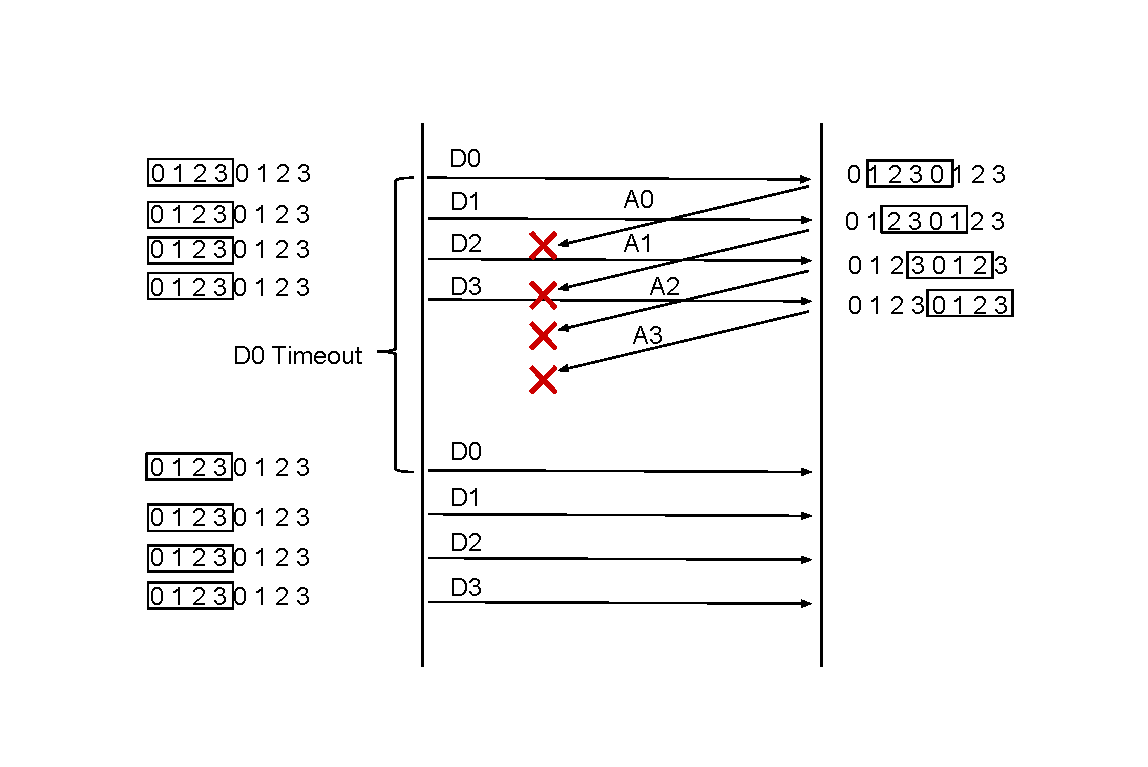
\includegraphics[width=\textwidth]{images/P7.pdf}
    \caption{FNC-TP problem}
    \label{fig:P7}
\end{figure}


%----------------------------------------------------------------------------------------
%	PROBLEM 8
%----------------------------------------------------------------------------------------

\section*{Problem 8}
(a).
Yes. This scheme is basically part of GBN. In terms of the TCP error control itself, it will work properly. However, consider that if a segment is missing, the sender needs to retransmit all the segments starting from the missing one. This is ineffecient in a high speed network and would yield low throughput. \\

(b).
Yes. This scheme is basically part of SR. It will work in terms of TCP error control. However, a problem in this scheme is also poor throughput. This really depends on how the ACK is implemented. If we make it do exactly what SR does, the sender would not be able retransmit a missing segment until timeout. This makes TCP go back to slow start every time, so the throughput is low. Additionally, if the timer is set inproperly in a high speed network, the sender's window cannot proceed without timeout. This could worsen the throughput. On the other hand, if the receiver uses cumulative ACK instead, this essentially becomes TCP Reno and will work just fine. \\

(c). \\
Advantage of (i): \\
1. Easy to implement, no need to worry about handling out-of-order segments. \\
2. Requires less resources, especially receiving buffer size. \\
Disadvantage of (i): \\
1. Poor throughput on a lossy path. \\

Advantage of (ii): \\
1. Reduces unnecessary retranmission, only retransmitts the lost segment. \\
Disadvantage of (ii): \\
1. More complicated to implement, needs to handle out-of-order segments. \\
2. Requires more space to buffer the out-of-order segments. \\


\end{document}
